\section{The mock catalog}
\label{sec:mock}

In this section we generate a photometric mock catalog $\lbrace m_j \pm \sigma_{m_j}, z,t \rbrace$ with observed magnitudes $m_j\pm\sigma_{m_j}$ in each PAU band $j$ for galaxies at redshift~$z$ and with spectral type~$t$.

\subsection{Noiseless magnitudes}
We use a method similar to that described in \citet{Jouvel2009}, which consists on sampling the cumulative Luminosity Function (LF): 
\begin{eqnarray}
N(z,t) = \int_{-\infty}^{M_{lim}(z,t)} \phi x^\alpha e^{-x} dx \nonumber \\
x\equiv10^{-0.4(M-M^*)},
\label{z_dist}
\end{eqnarray}
in the redshift range $z=[0,6]$, for a total of $N\sim10^6$ galaxies. $M$~is the absolute magnitude and $M_{lim}(z,t)$ the absolute magnitude limit at redshift $z$ and spectral type $t$ for a given apparent magnitude limit of the catalog $m_{lim}$ in some reference band. In our case $m_{lim}<26.0$ in the $r_{SDSS}$ band. Finally, $\lbrace M^*, \phi, \alpha \rbrace$ are the parameters of the LF, which also depend on $z$ and $t$. We assume that their redshift dependency is:
\begin{equation}
 \lbrace M^*, \log_{10}\phi, \alpha \rbrace = \lbrace a \exp[-(1+z)^{b}] + c \rbrace
\label{LF_param_evolv}
\end{equation}
where $\lbrace a, b, c \rbrace$ are type-dependent parameters whose values are in Table~\ref{LF_parameters}. These values are chosen to match the LFs and their evolution from \cite{Dahlen2005}, where three different spectral types, 1 = Elliptical (Ell), 2 = Spiral (Sp), 3 = Irregular (Irr), are distinguished. 
\begin{table*}
\centering
\caption{Parameters $\lbrace a,b,c \rbrace$ that, through (\ref{LF_param_evolv}), give the values and evolution in redshift of the LF parameters $\lbrace \log_{10}\phi, M^*, \alpha \rbrace$ for a given spectral type $t$. These values are based on the LFs in \citet{Dahlen2005}, where three galaxy types are distinguished: 1 = Ell, 2 = Sp and 3 = Irr.}
\vspace*{12pt}
\begin{tabular}{cccccccccc}
\cline{2-10}
& \multicolumn{3}{c}{$\log_{10}\phi$} & \multicolumn{3}{c}{$M^*$} & \multicolumn{3}{c}{$\alpha$}\\
\hline
\multicolumn{1}{c}{t} & a & b & c & a & b & c & a & b & c\\
\hline
\multicolumn{1}{c}{1} & 2.4 & 1.1 & -2.7 & 5.0 & 1.6 &-21.90 & 1.7 & 1.6 & -1.00 \\
\multicolumn{1}{c}{2} & 0.5 & 0.1 & -2.28 & 3.2 & 2.5 & -21.00 & 0.7 & -0.9 & -1.50 \\
\multicolumn{1}{c}{3} & 1.0 & -3.5 & -3.1 & 5.0 & 1.3 & -20.00 & 1.8 & 0.9 & -1.85 \\
\hline
\end{tabular}
\label{LF_parameters}
\end{table*}

The relation between the absolute magnitude $M$ and the apparent magnitude $m$ for a galaxy at redshift $z$ and with spectral type $t$, used in the magnitude limit of (\ref{z_dist}), is:
\begin{equation}
M =  m - 5 \log_{10}D_L(z) - 25 - K(z,t)
\label{abs_m}
\end{equation}
where $D_L(z)$ is the luminosity distance of the galaxy at redshift $z$ in Mpc, which in a flat $\Lambda$CDM universe is expressed as:
\begin{equation}
D_L(z) \equiv (1+z) {c \over H_0}\int_0^{z} {dz \over \sqrt{\Omega_M(1+z)^3 + \Omega_\Lambda} },
\end{equation}
with cosmological parameters chosen to be: $H_0$ = 75~(km/s)/Mpc, $\Omega_M$ = 0.25 and $\Omega_\Lambda$ = 0.75, and $K(z,t)$ is the $K$-correction:
\begin{equation}
K(z,t) \equiv -2.5 \log_{10} \left[{1 \over 1+z}{\int^{\infty}_{0} f_t(\lambda) R_0(\lambda)\lambda d\lambda  \over \int^{\infty}_{0} f_t((1+z)\lambda)R_0(\lambda)d\lambda}\right]
\end{equation}
where $R_0(\lambda)$ is the response of the reference band, $f_t(\lambda)$ is the Spectral Energy Density (SED) of the galaxy with spectral type $t$ in the rest frame, and $f_t((1+z)\lambda)$ the same SED at redshift $z$. As a representation of these SEDs, we use the \texttt{CWW} \citep{Coleman1980} extended template library from the \texttt{LePhare}\footnote{The extended \texttt{CWW} library can be found in the folder \tt{/lephare\_dev/sed/GAL/CE\_NEW/} of the \texttt{LePhare} package at \url{http://www.cfht.hawaii.edu/~arnouts/LEPHARE/DOWNLOAD/lephare\_dev\_v2.2.tar.gz}} photo-$z$ code. It contains 66 templates ranging through Ell$\rightarrow$Sp$\rightarrow$Irr and shown on Fig.~\ref{pau_templates}. We split them in three groups: Ell = (0-17), Sp = (17-55) and Irr = (55-66). Then, a specific template within one of these groups is randomly selected and assigned to the galaxy. Actually, we allow the spectral type $t$ to range from 1 to 66 with a resolution of 0.01 by interpolating between templates.
\begin{figure}
\centering
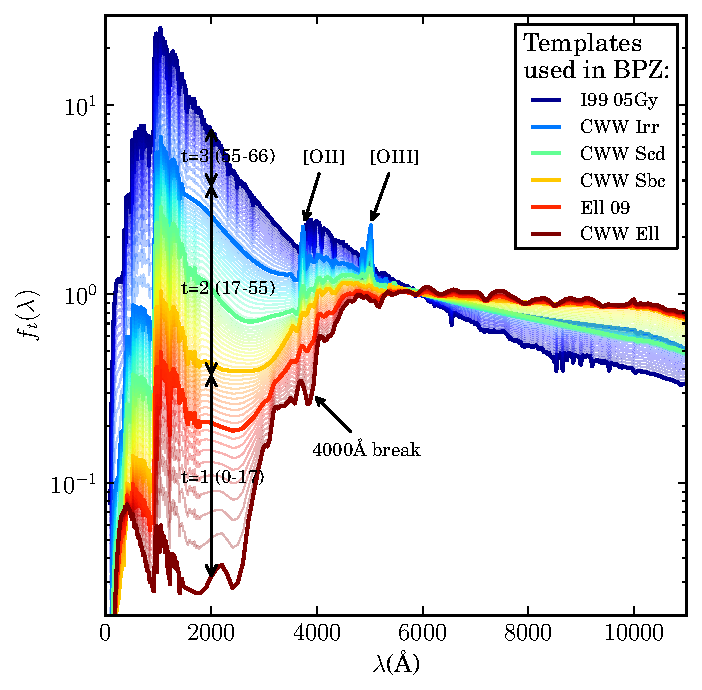
\includegraphics[width=84mm]{./plots/pau_templates.pdf}
\caption{The 66 spectral templates in the rest frame extracted from the extended CWW library. They are used, in (\ref{abs_m}) and (\ref{mi}), to generate the photometry of the PAU mock catalog. They evolve from Ellipticals (0-17, in red) to Spirals (17-55, in yellow, green and cyan), and finally to Irregulars (55-66, in blue and violet). Wider and deeper curves highlight the six templates used in \texttt{BPZ} to compute the photo-$z$s.}
\label{pau_templates}
\end{figure}

After assigning $\lbrace z,t \rbrace$ values for all galaxies, we also assign them an absolute magnitude $M$ randomly within the range $[-\infty, M_{lim}(z,t)]$ following the LF probability distribution in (\ref{z_dist}). Then, the apparent magnitude $m_0$, in our reference band $r_{SDSS}$, is computed from (\ref{abs_m}). The other magnitudes $m_j$ at any band $j$ are obtained through:
\begin{equation}
m_j = m_0 + 2.5 \log_{10} \left[ {\int^{\infty}_{0} f_t((1+z)\lambda) R_0(\lambda)\lambda d\lambda \over \int^{\infty}_{0} f_t((1+z)\lambda) R_j(\lambda)\lambda d\lambda} {\int^{\infty}_{0} R_j(\lambda) {d\lambda \over \lambda} \over \int^{\infty}_{0} R_0(\lambda) {d\lambda \over \lambda}}\right]
\label{mi}
\end{equation}
where $R_j(\lambda)$ is the response of some PAU band $j$.

\subsection{Noisy magnitudes}
The resulting magnitudes are noiseless, so we have to transform them to observed magnitudes by adding a random component of noise as follows:
\begin{equation}
m_j \rightarrow m_j + \eta(0,1)\sigma_{m_j},
\label{noiselesstonoisy}
\end{equation}
where $\eta(0,1)$ is a normal random variable and $\sigma_{m_j}$ the expected magnitude error which is related to the signal-to-noise in Eq.~(\ref{SN}) as follows:
\begin{equation}
\sigma_{m_j} = 2.5 \log_{10} \left(1 + {1 \over (S/N)_j} \right)
\label{errm}
\end{equation}
Additionally, we add an extra component of noise of size $\sim$0.022, corresponding to a $S/N=50$, in quadrature to $\sigma_m$, which takes into account some possible photometric calibration issues. Finally, we obtain the mock catalog $\lbrace m_j \pm \sigma_{m_j}, z,t \rbrace$. 

The resulting $\sigma_m$ vs. $m$ scatter plots, in the $i$ BB and the 7750\AA \ NB, are shown in Fig.~\ref{err_m}, where for the sake of clarity we only plot 10000 randomly selected galaxies. The 7750\AA \ band is chosen because its central wavelength is very similar to that of the $i$ band. Note how on both bands $\sigma_m$ starts being flat at $\sim$0.022 (the calibration error), and then, at fainter magnitudes, when the sky brightness and the CCD read-out noise become important, it grows and the scatter becomes wider. 
\begin{figure}
\centering
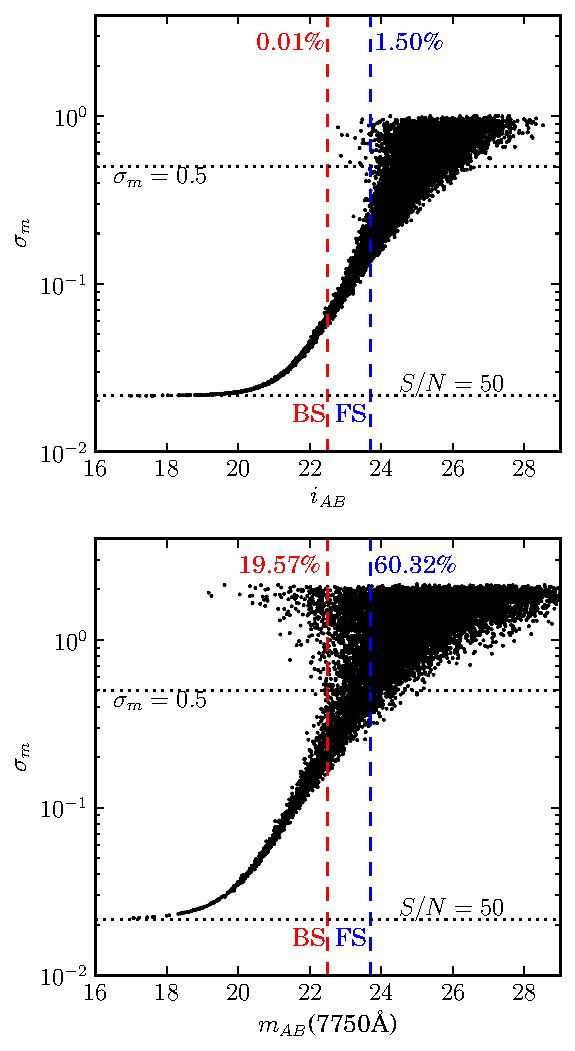
\includegraphics[width=80mm]{./plots/errm_pau.pdf}
\caption{Scatter plots of $\sigma_m$ vs. $m$ for the $i$ BB (top) and the 7750\AA \ NB (bottom). For the sake of clarity only 10000 randomly selected galaxies are plotted. The magnitude limits of the Bright Sample (BS; red) and Faint Sample (FS; blue) are also plotted as vertical-dashed lines. The bottom dotted line in both plots shows the calibration error ($S/N=50$) added in quadrature to $\sigma_m$, while the top dotted line shows the threshold where magnitudes are considered as non-observed. The fractions of non-observed magnitudes ($\sigma_m>0.5$) in each sample are also shown at the top with their corresponding color.}
\label{err_m}
\end{figure}

\subsection{Bright and Faint Samples}
The PAU survey science will be mostly focused on Large Scale Structure (LSS) studies such as cross measurements of Redshift Space Distortions (RSD) and Magnification Bias (MAG) between two galaxy samples: the Bright Sample (BS) on the foreground and the Faint Sample (FS) on the background (see \cite{Gaztanaga2012}). The BS should contain galaxies bright enough to have a large signal-to-noise in all bands, including the narrow bands, and, therefore, reach the necessary photo-$z$ accuracy to measure RSD. 
We see in Fig.~\ref{pau_lim_mag} that the 5-$\sigma$ limiting magnitudes for the NB are close to 22.5, so we define the BS as all those galaxies with $i_{AB} \equiv m_{AB}(i)<22.5$. The FS will contain the rest of the galaxies within $22.5<i_{AB}<23.7$. The upper limit has been chosen to roughly match the 5-$\sigma$ limiting magnitudes of the broad bands (see Fig.~\ref{pau_lim_mag}). 
We consider that a magnitude is not observed in one band if its corresponding error is $\sigma_{m}>0.5$. We find that a $\sim$0.01\% of galaxies in the BS are not observed in the $i$ band, with the fraction increasing to $\sim$1.5\% in the FS. Similarly, in the BS $\sim$19.57\% are not observed in the 7750\AA \ band, increasing to $\sim$60.32\% in the FS (see Fig.~\ref{err_m}). This tells us that, while most of the BB information will be present in both samples, the presence of NB information in the FS will be rather limited, degrading considerably the photo-$z$s. %However, part of these FS galaxies will be the magnified sources for MAG and they can afford a poorer photo-$z$ quality according to \cite{Gaztanaga2012}.

In Fig.~\ref{mzt_dist} we show the resulting distributions of the magnitude $i_{AB}$ (top-left), the true redshift $z$ (top-right) and the spectral type $t$ (bottom) of the galaxies in the whole catalog (black-dotted), the BS (red-solid) and the FS (blue-solid). The magnitude distribution of the whole catalog has its maximum at $\sim$25.0, so that the BS and FS are on the brighter tail of the distribution and account for $\sim$8.4\% and $\sim$13\% of the whole catalog respectively. However, this also helps both samples to have a very good completeness up to their magnitude limit. We can also see that, while the whole catalog extends up to $z\sim5$, the BS only goes up to $z\sim1.5$ and the FS up to $z\sim3$. Finally, we see that both BS and FS have a similar proportion of Spiral galaxies ($t=2$), $\sim55$\%; however the BS contains more elliptical galaxies (33\%) than the FS (19\%), and consequently, the FS contains more irregular galaxies. 

\begin{figure*}
\centering
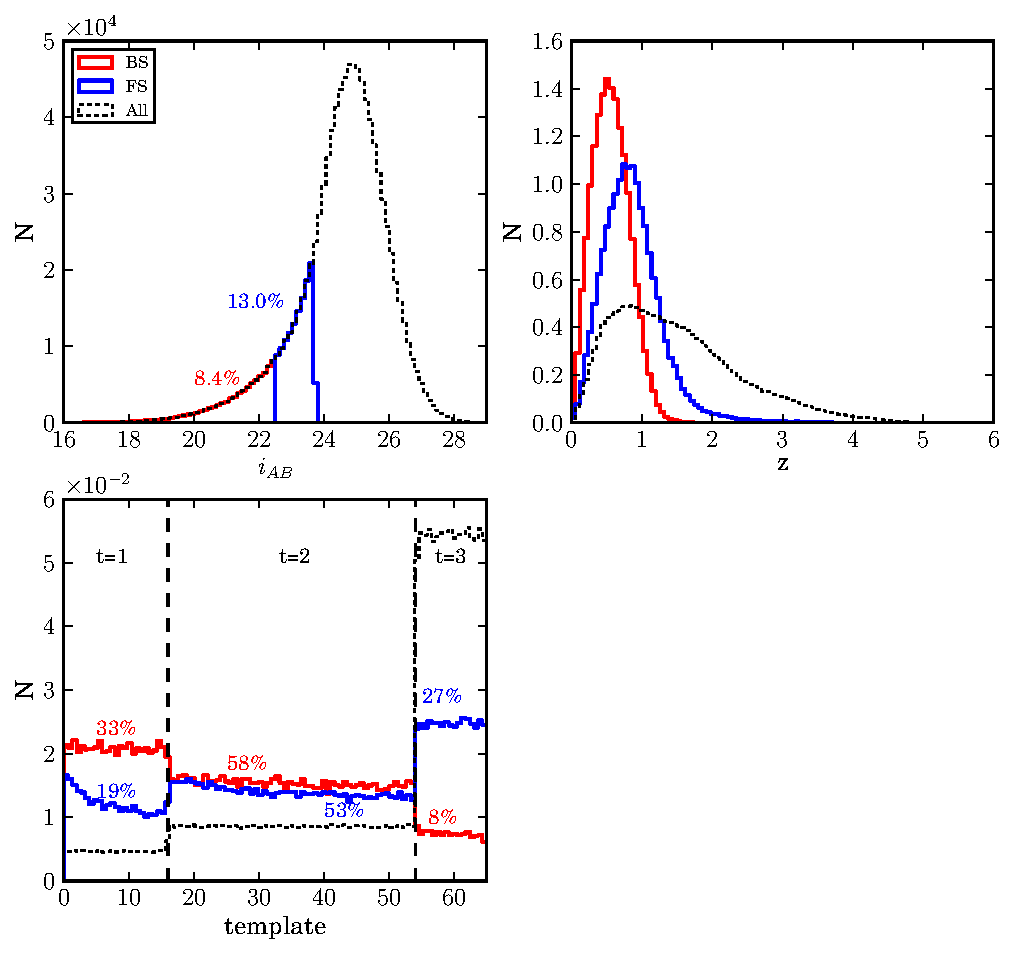
\includegraphics[width=130mm]{./plots/mzt_pau.pdf}
\caption{The observed magnitude in the $i$ band (top-left), true redshift (top-right) and spectral type distributions for the whole catalog (black), the BS $i_{AB}<22.5$ (red) and the FS $22.5<i_{AB}<23.7$ (blue). We also show the fraction of the total galaxies in each sample in the magnitude distribution plot, in their corresponding color. Similarly, we show the proportions of spectral types in each sample. The redshift and type distributions have been normalized.}
\label{mzt_dist}
\end{figure*}
